\documentclass[11pt]{article}
\usepackage{amsmath,amsthm,amssymb,fullpage,graphicx,hyperref}
\usepackage{listings,color,setspace}
\usepackage{titling}
\usepackage{setspace}
%% \usepackage{cite}
\usepackage{natbib}
\newcommand{\subtitle}[1]{%
  \posttitle{%
    \par\end{center}
    \begin{center}\large#1\end{center}
    \vskip0.5em}%
}

\author{Andy Reagan}
\subtitle{Math 337 Final Project Handout}
\title{Algorithmic Differentiation}

     \def\NN{\mathbb{N} }
     \def\ZZ{\mathbb{Z} }
     \def\QQ{\mathbb{Q} }
     \def\RR{\mathbb{R} }
     \def\CC{\mathbb{C} }
     \def\f{\frac }
     \def\b{\begin }
     \def\e{\end }
     \def\Log{\text{Log} \,}
     \def\Re{\text{Re} \, }
     \newcommand{\pdiff}[2]{\frac{\partial #1}{\partial #2}}
     \newcommand{\partialdiff}[2]{\frac{\partial #1}{\partial #2}}
     \newcommand{\pdiffsq}[2]{\frac{\partial^2 #1}{{\partial #2}^2}}
     \newcommand{\pdiffcu}[2]{\frac{\partial^3 #1}{{\partial #2}^3}}
     \newcommand{\pdiffhi}[3]{\frac{\partial^#3 #1}{{\partial #2}^#3}}
     \newcommand{\diff}[2]{\frac{{\rm d}#1}{{\rm d}#2}}
     \newcommand{\diffsq}[2]{\frac{{\rm d}^{2}#1}{{\rm d} {#2}^2}}
     \newcommand{\diffhi}[3]{\frac{{\rm d}^#3 #1}{{\rm d} {#2}^#3}}
     \newcommand{\tdiff}[2]{\mbox{d} #1/\mbox{d} #2}
     \newcommand{\tdiffsq}[2]{\mbox{d}^{2} #1/\mbox{d} {#2}^2}
     \newcommand{\tpdiff}[2]{\partial #1/\partial #2}
     \newcommand{\tpdiffsq}[2]{\partial^2 #1/\partial {#2}^2}
     \newcommand{\bvec}[1]{\vec{ {\bf #1 } }}
     \newcommand{\oh}[1]{O(h^{{#1}})}

\newtheorem{theorem}{Theorem}[section]
\newtheorem{lemma}[theorem]{Lemma}
\newtheorem{proposition}[theorem]{Proposition}
\newtheorem{corollary}[theorem]{Corollary}

%% \newenvironment{proof}[1][Proof]{\begin{trivlist}
%% \item[\hskip \labelsep {\bfseries #1}]}{\end{trivlist}}
%% \newenvironment{definition}[1][Definition]{\begin{trivlist}
%% \item[\hskip \labelsep {\bfseries #1}]}{\end{trivlist}}
%% \newenvironment{example}[1][Example]{\begin{trivlist}
%% \item[\hskip \labelsep {\bfseries #1}]}{\end{trivlist}}
\newenvironment{remark}[1][Remark]{\begin{trivlist}
\item[\hskip \labelsep {\bfseries #1}]}{\end{trivlist}}

%% \newcommand{\qed}{\nobreak \ifvmode \relax \else
%%       \ifdim\lastskip<1.5em \hskip-\lastskip
%%       \hskip1.5em plus0em minus0.5em \fi \nobreak
%%       \vrule height0.75em width0.5em depth0.25em\fi}

\lstset{language=MATLAB,
basicstyle=\ttfamily\scriptsize\singlespacing,
keywordstyle=\color{black},
stringstyle=\color{black},
commentstyle=\color{black},
morecomment=[l][\color{black}]{\#},
frame=L,
xleftmargin=\parindent,
%%numbers=left,                   %% where to put the line-numbers
%%numberstyle=\scriptsize,      %% the size of the fonts that are used for the line-numbers
%%stepnumber=1,                   %% the step between two line-numbers. If it is 1 each line will be numbered
numbersep=5pt,
breaklines=true,        %% sets automatic line breaking
breakatwhitespace=false,    %% sets if automatic breaks should only happen at whitespace
escapeinside={\%*}{*)} 
}

\linespread{1.5}

%% example code insert
%% \lstinputlisting[language=Matlab]{andy_hw12_prb01.m}

%% example figure
%% \begin{figure}[h!]
%%   \centering
%%     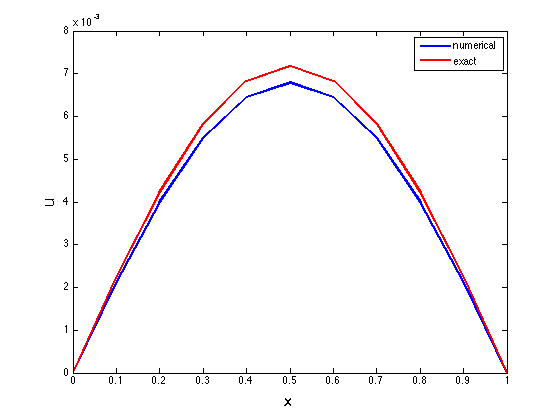
\includegraphics[width=0.45\textwidth]{andy_hw12_prb01_02.png}
%%   \caption{The numerical and exact solution for $h=0.1$.}
%% \end{figure}

%% start problem on next page
%% \clearpage
%% \pagebreak

\begin{document}
% \vspace{1cm}

\maketitle

\pagebreak
\tableofcontents

\pagebreak
\section{Introduction}

The key question that we attempt to answer when modeling real-world phenomena is: how sensitive is the output of model with respect to the input values and parameters?
Most of the methods that we have developed in the class rely on finite differences to answer this question, and hence to make accurate predictions.
We judge the accuracy of these methods based on how well they approximate the Taylor series of the given function, giving rise to their local truncation error.
Accuracy is not the sole desired property of a numerical scheme, but once convergence to the true solution can be achieved, we seek the most efficient and most accurate determination of this solution.

A promising tool to answer the above question, with arbitrary accuracy, support for extended precision arithmetic, and the ability to apply to comlex, large-scale models is Algorithmic Differentiation. 
My presentation today outlines the basics of Algorithmic Differentation (AD) technology.
Some of the literature refers to AD as Automatic Differentiation, but in my experience the differentiation is still far from automatic.

The core functionality of AD relies upon the fact that any computer program can be broken down into a sequence of elementary operations, for which the derivative can be computed easily.
One limitation of this approach is that we are restricted to a range of functions that can be broken down this way, although we will see that this is not as limiting in practical implementations.
There are many ways to potentially compute derivatives algorithmically, and we will discuss source code transformation, derivative compilers, and operator overloading techniques.

\subsection{Taylor Method}

Going back to Day 1, we are interesting in solving problems of the form of Eq (0.1) of the notes:
\[ y'(x) = f(x,y) .\]
Instead of taking the finite difference, we next consider the Taylor series expansion:
\begin{align*} f(x,y) = f(x_0,y_0) &+ \left (\Delta x f_x (x_0,y_0)+ \Delta y f_y (x_0,y_0)\right ) \\
&+ \f{1}{2!} \left ( \left ( \Delta x\right ) ^2 f_{xx} (x_0,y_0) + 2\Delta x \Delta y f_{xy} (x_0,y_0) + \left ( \Delta y \right ) ^2 f_{yy} (x_0,y_0) \right ) + \ldots \end{align*}

The computation of the forms of $f_x,f_y$ and so forth requires significantly effort from a computer, and will typically be cumbersome.
Therefore, evaluating them will be slow.
Algorithm differentiation overcomes this difficulty.
We will discuss this in more detail in the following section.

\pagebreak
\section{Algorithmic Differentiation Basics}

First I will note other possibilities for computing derivatives and jacobians, namely: symbolic differentiation, hand-coding, and divided differences.
In line with the goals of \cite{bischof2000computing}, we seek to evaluate derivatives in a way that has the following properties:
\begin{itemize}
\item {\bf Reliability} The computed derivatives should be accurate to the IEEE floating point arithmetic of the computer.
\item {\bf Computational Cost} Computing the derivatives is often the main computational cost. The amount of memory and operations should be bounded.
\item {\bf Scalability} The approach should give correct results for a 1-line formula as well as a 100,000-line code.
\item {\bf Human Effort} A user should not spend much time preparing a code for differentiation, in particular where code changes frequently.
\end{itemize}

Handcoding, divided-difference approximations, and symbolic manipulators fall short with respect to the previously mentioned criteria. The main drawbacks of divided-difference approximations are their numerical unpredictability and their computational cost. 
In contrast, both the handcoding and symbolic approaches suffer from a lack of scalability and require considerable human effort \cite{bischof2000computing}.

To simplify the discussion, I adopt the notation of \cite{jorba2005software}.
If $a : t \in I \subset \RR \to \RR$ is a smooth function, denote its normalized $n$-th derivative to the value
\[ a^{[n]} (t) = \f{1}{n!} a ^{(n)} (t) .\]
Assume now that $a(t) = F(b(t),c(t))$ and that we know the values of $b^{[j]} (t)$ and $c^{[j]} (t)$, $j= 0,\ldots, n$ for a given $t$.
I will prove the following on the board:
\begin{proposition} If the function $a$ and $b$ are of class $C^n$, and $\alpha \in \{ \RR - 0 \}$, we have
\begin{enumerate}
\item If $a(t) = b(t) \pm c(t) $, then $a^{[n]}(t) = b^{[t]}(t) \pm c^{[t]}(t).$
\item If $a(t) = b(t) c(t) $, then $a^{[n]}(t) = \sum _{j=0} ^n b^{[n-j]}(t) c^{[j]}(t).$
\item If $a(t) = \f{b(t)}{ c(t)} $, then $a^{[n]}(t) =  \f{1}{ c^{[0]}(t)} \left [ b^{[n]}(t) - \sum _{j=1} ^n c^{[j]}(t) a^{[n-j]}(t) \right ].$
\item If $a(t) = b(t)^{\alpha } $, then $a^{[n]}(t) =  \f{1}{ nb^{[0]}(t)} \sum _{j=0} ^{n-1} \left ( n \alpha - j(\alpha +1 ) \right ) b^{[n-j]}(t) a^{[j]}(t).$
\item If $a(t) = e^{b(t)}$, then $a^{[n]}(t) =  \f{1}{ n} \sum _{j=0} ^{n-1} \left ( n - j \right ) b^{[n-j]}(t) a^{[j]}(t).$
\item If $a(t) = \ln b(t)$, then $a^{[n]}(t) =  \f{1}{ b^{[0]}(t)} \left [ n^{[n]} (t) - \f{1}{n} \sum _{j=1} ^{n-1} \left ( n - j \right ) b^{[j]}(t) a^{[n-j]}(t) \right ].$
\item If $a(t) = \cos c(t)$ and $b(t) = \sin c(t)$, then 
\[a^{[n]}(t) =  -\f{1}{ n} \sum _{j=1} ^{n} j b^{[n-j]}(t) c^{[j]}(t),~~~~b^{[n]}(t) =  \f{1}{ n} \sum _{j=1} ^{n} j a^{[n-j]}(t) c^{[j]}(t) .\]
\end{enumerate}
\label{pr:mainprop}
\end{proposition}

\begin{remark} It is possible to derive similar forumulas for other functions, line inverse trigonometric functions.
\end{remark}

\begin{corollary} The number of arithmetic operations to evaluate the normalized derivation of a function up to order $n$ is $O(n^2)$.
\end{corollary}

I will prove this on the board as well.

\subsection{Short Example}
I base my example on that of \cite{jorba2005software}, and apply the rules of Proposition \ref{pr:mainprop} to the Van der Pol equation:
\begin{align*} x' &= y\\
y' &= (1-x^2)y -x \end{align*}
We decompose this function in the following elementary operations:
\begin{align*}
u_1 &= x\\
u_2 &= y\\
u_3 &= u_1u_1\\
u_4 &= 1 - u_3\\
u_5 &= u_2u_4\\
u_6 &= u_5 - u_1\\
x' &= u_2\\
y' &= u_6\end{align*}

And applying Proposition \ref{pr:mainprop} to the above, we have
\begin{align*}
u_1^{[n]}(t) &= x^{[n]}(t)\\
u_2^{[n]}(t) &= y^{[n]}(t)\\
u_3^{[n]}(t) &= \sum _{i=0} ^n u_1^{[n-i]}(t)u_1^{[i]}(t)\\
u_4^{[n]}(t) &= 1 - u_3^{[n]}(t)\\
u_5^{[n]}(t) &= \sum _{i=0} ^n u_2^{[n-i]}(t)u_4^{[i]}(t)\\
u_6^{[n]}(t) &= u_5^{[n]}(t) - u_1^{[n]}(t)\\
x^{[n+1]}(t) &= \f{1}{n+1}u_2^{[n]}(t)\\
y^{[n+1]}(t) &= \f{1}{n+1}u_6^{[n]}(t)\end{align*}

\subsection{High accuracy computations}

To achieve a given level of accuracy, we can choose both the step size $h$ and the order $p$.
Of course, we need to be cognizant of the radius of covergence of the power series we create and the effect that this has on the stability of the step.
Since we can control both order and step size, we attempt the dual goals of the desired accuracy and efficient computation.



\pagebreak
\section{Using Taylor 1.4}

Taylor 1.4 is a package that is specifically designed to use AD to integrate systems of equations.
The documentation for the package is excellent, in both an extended paper \cite{jorba2005software}, and an online appendix (\url{http://www.ma.utexas.edu/users/mzou/taylor/manual/manual.html}).
I downloaded and built the software using \verb|gcc|, specifically

\lstinputlisting[language=Bash]{code/Taylor1.4/gccv.txt}

I specify the Kepler two-body problem as

\lstinputlisting[language=Bash]{code/Taylor1.4/tbp.in}

and build the executable with

\lstinputlisting[language=Bash]{code/Taylor1.4/make.sh}

\pagebreak
\section{Comparison to Symplectic Methods}

We perform tests with the Kepler two-body problem (Eq (5.30) of the notes):
  \[ q'' = - \f{q}{(q^2+r^2)^{3/2}} ~~,~~~~~r'' = - \f{r}{(q^2+r^2)^{3/2}};  \]
where $q$ and $r$ are the cartesian coordinates of a certain radius vector relative to the center of mass of the bodies.

Although we could solve this directly, we first put the problem into a system of four ODE's:
\begin{align*} z' &= -\f{q}{(q^2+r^2)^{3/2}} \\
               w' &= - \f{r}{(q^2+r^2)^{3/2}} \\
               q' &= z\\
               r' &= w.\end{align*}

For comparison, we apply the Verlet-1 and -2 methods to the Kepler two-body problem.
We start with $h = 0.1$ and $t_{\max} =  500$, and decrease $h$ to preserve the Runge-Lenz vector.
As the initial condition, use
\[ q(0) = 1-\text{ecc}, ~~~r(0) = 0,~~~Q(0) = 0, ~~~ R(0) = \sqrt{\f{1+\text{ecc}}{1-\text{ecc}}} ~~~\text{for}~ \text{ecc} = 0.6,\]
which corresponds to the exact solution being an elipse with eccentricity 0.6.
As we observed in HW5, Bonus 2, the Verlet method loses the orientation of the orbit for large $h$.
Here are three plots for varying $h$, starting at $0.1$ down the $0.005$, where the orbit appears to stick around.
I didn't spend a long time optimizing the MATLAB code, and it takes quite a long time to run (without making plots):
\lstinputlisting[language=Bash]{code/MATLAB/outputtime.txt}

\begin{figure}[h!]
  \centering
  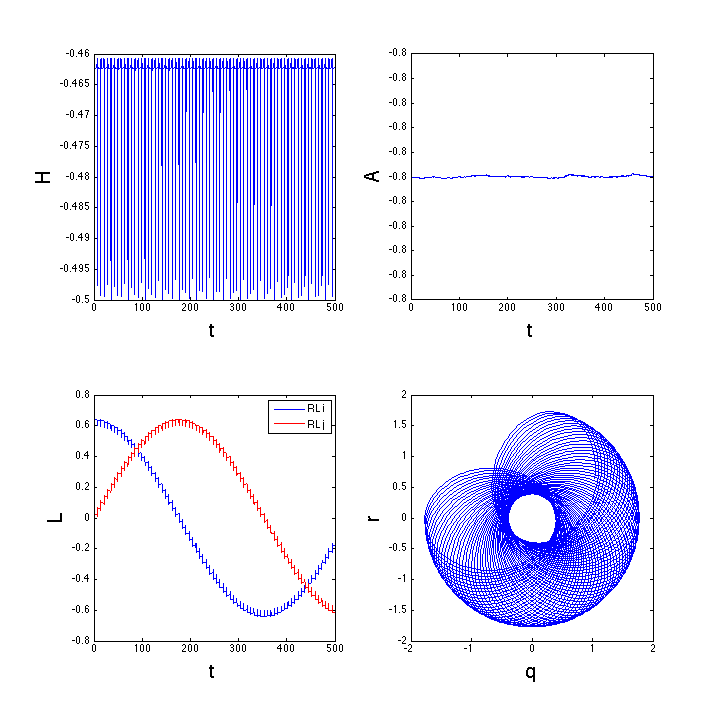
\includegraphics[width=0.75\textwidth]{code/MATLAB/andy_hw12_01.png}
  \caption{The numerical solution for $h=0.1$.
  In the top left panel we plot the Hamiltonian, top right the angular momentum, bottom left the Runge-Lenz vector, and bottom right the phase space plot.}
\end{figure}

\begin{figure}[h!]
  \centering
  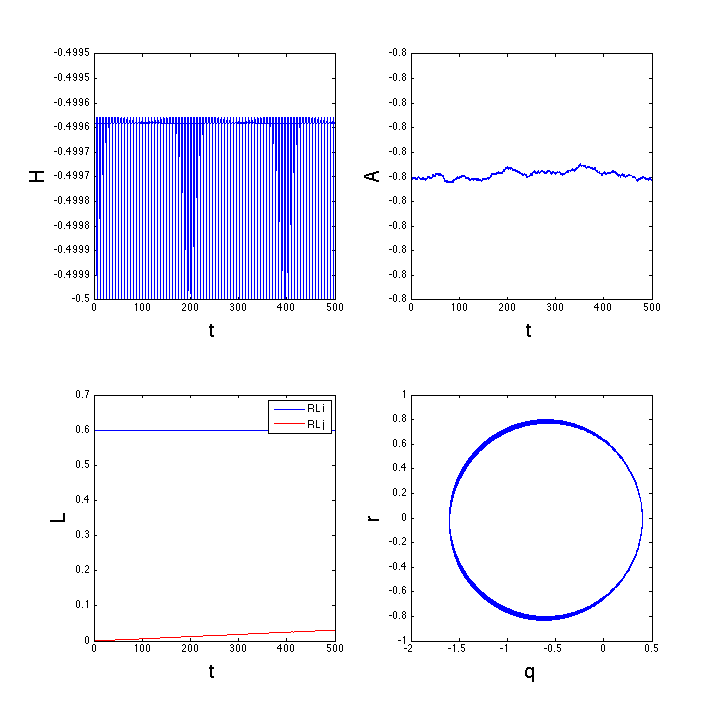
\includegraphics[width=0.75\textwidth]{code/MATLAB/andy_hw12_02.png}
  \caption{The numerical solution for $h=0.01$.
  In the top left panel we plot the Hamiltonian, top right the angular momentum, bottom left the Runge-Lenz vector, and bottom right the phase space plot.}
\end{figure}

\begin{figure}[h!]
  \centering
  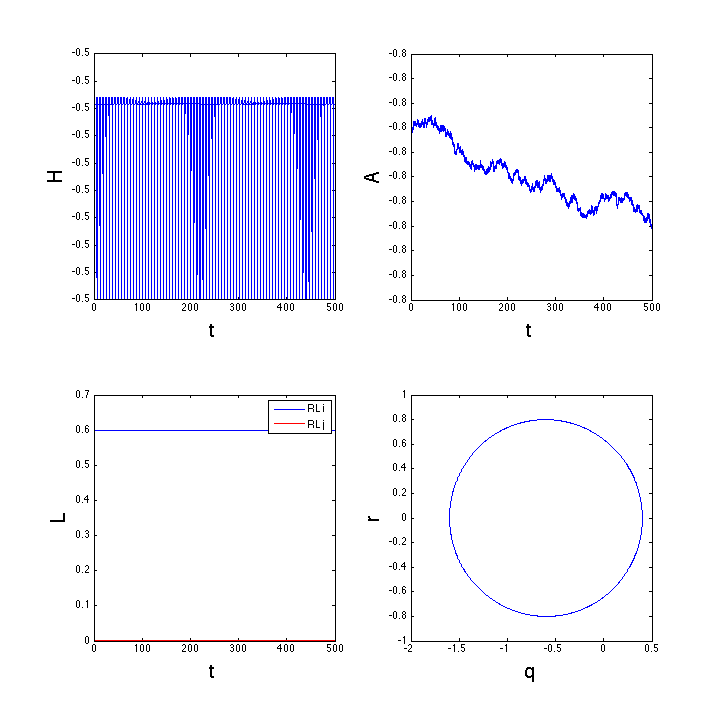
\includegraphics[width=0.75\textwidth]{code/MATLAB/andy_hw12_03.png}
  \caption{The numerical solution for $h=0.001$.
  In the top left panel we plot the Hamiltonian, top right the angular momentum, bottom left the Runge-Lenz vector, and bottom right the phase space plot.}
\end{figure}

\clearpage
\pagebreak
%% Loading the output files from the ANSI C routine generated by Taylor 1.4 into MATLAB is difficult.
To visualize the output of the ANSI C routine generated by Taylor 1.4 we import the data file into Python, and plot the orbit.
The calculation is nearly immediate with Taylor 1.4:
\lstinputlisting[language=Bash]{code/Taylor1.4/outputtime.txt}

The plot of this solution is:
\begin{figure}[h!]
  \centering
    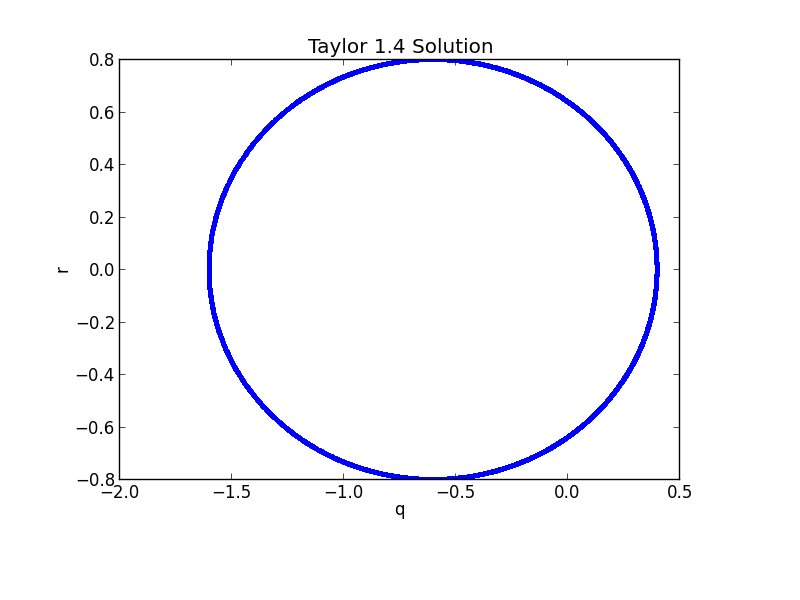
\includegraphics[width=0.85\textwidth]{code/Taylor1.4/figures/test.png}
  \caption{Solution with the Taylor method.}
\end{figure}

Directly comparing the endpoint of the calculation, for MATLAB we have:
\lstinputlisting[language=Bash]{code/MATLAB/end.txt}
and from Taylor we have:
\lstinputlisting[language=Bash]{code/Taylor1.4/end.txt}

Of course, we can't really be sure that this means that the solutions are the same, because the orbit is periodic (one could have simply lapped the other!).

\pagebreak
\section{Conclusions}

It took a long time to figure out how to get the code to run, again confirming that the process is not automatic, however the speed with which the high accuracy simulation can be coded and computed is impressive.
As AD continues to gain popularity, the use cases will grow beyond those in traditional optimization.
With the ability to solve equations with arbitrary accuracy (extended precision arithmetic), more research may find applications for the Taylor method.




\pagebreak
\nocite{bischof2000computing}
\nocite{gay2006semiautomatic}
\nocite{griewank2003mathematical}
\nocite{pryce2008fast}
\nocite{barrio2005performance}
\nocite{jorba2005software}
\nocite{verma2000introduction}
\nocite{walther2012getting}

\bibliographystyle{chicago}
\bibliography{337_final}

\end{document}



